% PLEASE USE THIS FILE AS A TEMPLATE
% Check file iosart2x.tex for more examples

% add. options: [seceqn,secthm,crcready,onecolumn]
\documentclass[sw]{iosart2x}

%\usepackage{dcolumn}
%\usepackage{endnotes}

%para el simbolo de chequeado
\usepackage{amssymb}% http://ctan.org/pkg/amssymb
\usepackage{pifont}% http://ctan.org/pkg/pifont
\usepackage{xcolor}
\newcommand{\cmark}{\ding{51}}%
\newcommand{\xmark}{\ding{55}}%

\newcommand{\am}[1]{{\color{green!50!black}\textsc{am:} #1}}
\newcommand{\ah}[1]{{\color{blue!70!black}\textsc{ah:} #1}}
\newcommand{\li}[1]{{\color{red!50!black}\textsc{am:} #1}}

%%%%%%%%%%% Put your definitions here
\newtheorem{example}{Example}

%%%%%%%%%%% End of definitions

\pubyear{0000}
\volume{0}
\firstpage{1}
\lastpage{1}

\begin{document}

\begin{frontmatter}

%\pretitle{}
\title{Consuming Dynamic Linked Data Knowledge Graphs: A Survey}
\runningtitle{Consuming Dynamic Linked Data Knowledge Graphs: A Survey}

% Two or more authors:
\author[A]{\inits{A.}\fnms{Alberto} \snm{Moya Loustaunau}\ead[label=e1]{amoya@dcc.uchile.cl}},
\author[B]{\inits{L.-D.}\fnms{Luis-Daniel} \snm{Ibáñez}\ead[label=e2]{l.d.ibanez@soton.ac.uk}}
and
\author[A]{\inits{N.N.}\fnms{Aidan} \snm{Hogan}\ead[label=e3]{ahogan@dcc.uchile.cl}}
\runningauthor{A. Moya et al.}
\address[A]{IMFD Chile; Department of Computer Science, \orgname{University of Chile}, \cny{Chile}\printead[presep={\\}]{e1,e3}}
\address[B]{\orgname{University of Southampton},
Southampton, \cny{UK}\printead[presep={\\}]{e2}}

\begin{abstract}
A number of prominent open knowledge graphs have been published as Linked Data. These knowledge graphs are dynamic: the resources described by these graphs are continuously created, moved, modified, deleted, linked, and unlinked. Applications that consume data from such knowledge graphs must take these changes into account in order to deliver accurate services over up-to-date data. However, keeping track of such changes can be a costly process, particularly for multiple remote knowledge graphs accessible over the Web. This challenge has been acknowledged by a variety of researchers who have responded by suggesting techniques for dealing with dynamic knowledge graphs, but the current understanding of this problem is still incomplete. Our contribution is a systematic literature review on techniques for consuming dynamic knowledge graphs in a Linked Data setting, identifying respective potentials and limits. \ah{Revise/extend later.}
\end{abstract}

\begin{keyword}
\kwd{Data Dynamics}
\kwd{Knowledge Graphs}
\kwd{Linked Data}
\end{keyword}

\end{frontmatter}

%%%%%%%%%%% The article body starts:

\section{Introduction}\label{Introduction}

%\textbf{Contex}: 

The Semantic Web (SW) initiative aims to enable the automation of increasingly complex tasks using the Web through the provision of increasingly machine readable content on the Web~\cite{semwebsa}. The W3C\footnote{World Wide Web Consortium: https://www.w3.org/ } has recommended a variety of SW standards towards this goal. The core SW standard is the Resource Description Framework (RDF)~\cite{rdfconcepts11}, which outlines a graph-based data model by which the content of the Web can be structured and interlinked. Another key standard is the SPARQL Protocol and RDF Query Language (SPARQL)~\cite{sparql11}, which can be used for expressing potentially complex queries over RDF. Other standards include RDF Schema (RDFS)~\cite{rdfschema11} and the Web Ontology Language (OWL)~\cite{owl2primer} for defining the semantics of terms used in the RDF graph, and the Shapes Constraint Language (SHACL)~\cite{shacl} for validating RDF graphs with respect to specified constraints.

The Linked Data (LD) principles and best practices then outline a set of guidelines for publishing and interlinking RDF content on the Web in a decentralized manner~\cite{ldbook}. Linked Open Data (LOD) refers to the publication of data following LD principles on the Web under an open license. Supporting these initiatives, the LD community has developed -- and continues to develop -- novel techniques and tools for generating~\cite{Bizer03,GentileZC15}, publishing~\cite{CorlosquetDCPD09,MaaliCP12}, interlinking~\cite{silk,NgomoA11}, querying~\cite{HartigBF09,VerborghSHHVMHC16} and otherwise consuming~\cite{TummarelloDO07,swsejws} LD. A growing number of publishers, in a variety of different domains~\cite{SchmachtenbergBP14}, have contributed to the LOD ecosystem over the years. In order to visualize this growing ecosystem, the LOD Cloud\footnote{\url{http://lod-cloud.net}; McCrae et al.} depicts a graph of Linked Open Datasets and their interconnections, where it describes 1,255 datasets as of May 2020; some of the largest of these datasets provide RDF descriptions of millions of resources~\cite{ErxlebenGKMV14,dbpedia}. Syntaxes for RDF have also become common for schema.org markup~\cite{schemaorg}, being used on millions of websites~\cite{MeuselPB14}.
These developments have given rise to the first concrete instance of a so-called Web of Data (WoD)~\cite{wodbook}: a Web composed of structured, interlinked data.

More recently, the concept of a ``knowledge graph'' has been gaining traction, in particular, after the announcement of the Google Knowledge Graph~\cite{GoogleKG}, followed by further announcements by companies such as eBay, Facebook IBM, Microsoft~\cite{NoyGJNPT19} and many more besides. While many so-called ``enterprise knowledge graphs'' are proprietary and thus internal to a particular organization~\cite{NoyGJNPT19}, other so-called ``open knowledge graphs'' are published on the Web under open licenses for the common good~\cite{FarberBMR18}. Prominent examples of open knowledge graphs include BabelNet~\cite{NavigliP12}, DBpedia~\cite{dbpedia}, OpenCyc~\cite{FarberBMR18}, Wikidata~\cite{VrandecicK14} and YAGO~\cite{HoffartSBW13}. Leveraging RDF as a standard graph-structured data model, most such open knowledge graphs are published using the Semantic Web standards and the Linked Data principles~\cite{FarberBMR18,MalyshevKGGB18}, thus forming an integral part of the Web of Data. The most prominent such knowledge graphs receive upwards of millions of queries per data over the Web~\cite{SaleemAHMN15,MalyshevKGGB18}.
\medskip

Rather than being static, open knowledge graphs are subject to continuous change, and the broader Web of Data is further subject to expansion in size, scope and diversity, with new datasets being added, and obsolete ones being removed~\cite{UmbrichHHPD10, AuerDML12, KaferAUOH13, DividinoSGG13, SchmachtenbergBP14}. This creates a challenge for the applications that both manage and consume this data: how to deal with dynamic knowledge graphs on the Web? Without adequate techniques to deal with the aforementioned changes in open knowledge graphs, applications may succumb to a variety of undesirable outcomes~\cite{MeimarisPPGS14}: they may return results that are no longer valid, they may omit new information, they may miss relevant sources of data that have recently been added, they may link to sources of data that are no longer available, and so forth. This survey focuses on the challenge of consuming dynamic knowledge graphs published as Linked Data.
\medskip

% AH: cannot find the BancilhonDK92 reference. Is it relevant?

The challenge of managing dynamic data in an effective manner is not unique to this particular setting. Various works have addressed related issues in the context of relational databases, in terms of database reorganization~\cite{LernerH90}, schema versioning~\cite{Roddick95}, view maintenance~\cite{GuptaM95}, among other topics; however, such works address the problem of dynamics in a local setting, whereas the decentralized nature of Linked Data poses non-trivial challenges. Researchers have also investigated dynamics in the context of the traditional Web, proposing techniques relating to incremental crawling~\cite{ChoG00}, Web caching~\cite{GaddeCR01}, dynamic information retrieval~\cite{RisvikM02}, change frequency estimations~\cite{ChoG03}, user behavior~\cite{AlmeidaMC07}, and more besides; however, these latter works focus on the dynamics of mostly unstructured content (text), whereas Linked Data is structured.

While approaches for dealing with the dynamics of Linked Data can -- as we will see in this survey -- potentially borrow insights from the techniques and results developed in the context of relational databases~\cite{LernerH90,Roddick95,GuptaM95} and the Web~\cite{ChoG00,GaddeCR01,RisvikM02,ChoG03,AlmeidaMC07}, the combination of decentralization and structured data inherent to Linked Data implies unique challenges (and opportunities) with respect to dynamics, which can benefit from bespoke techniques that go beyond a straightforward synthesis of the state-of-the-art from other related areas.
\medskip

In the past years, a number of works have proposed bespoke concepts and techniques to address the inherent challenges of handling dynamic Linked Data. An important milestone was the initiation in 2010 of the W3C Dataset Dynamics Interest Group\footnote{https://www.w3.org/wiki/DatasetDynamics}: a community effort to study the dynamics of individual Linked Datasets and the broader Web of Data, motivated by the emergent challenges that were observed at that time. The community group at that time provided a brief survey of tools and techniques that could be brought to bear for taming dynamic Linked Data, including methods for link maintenance~\cite{PopitschH10,PopitschH11}, notification mechanisms~\cite{TrampFEA10}, subscription mechanisms~\cite{Fitzpatrick10,PassantM10}, change frequency~\cite{UmbrichHHPD10}, and more besides. A concise survey of these developments was provided by Umbrich et al.~\cite{UmbrichVH10} at that time. Since then a much broader range of works have emerged on the topic, investigating further aspects including archiving~\cite{UmbrichMP15}, caching mechanisms~\cite{MartinUA10,LampoVDR11,UmbrichKHP12,DehghanzadehPKUHD14,DividinoGS15,Kjernsmo15,ZhangSTQ15,NishiokaS17,dehghanzadeh2017}, change detection~\cite{ZeginisTC11,PapavasileiouFFKC13,DividinoKG14,PernelleSMT16}, change prediction~\cite{GonzalezH18,LoustaunauH19}, change verification~\cite{NishiokaS18}, continuous querying~\cite{DehghanzadehDGV15}, dynamic observatories~\cite{KaferUHP12}, synchronization~\cite{KnuthHS16,TummarelloMBE07}, versioning~\cite{GraubeHU14}, vocabularies~\cite{Berners04,Dady10} as well as more general works aiming to analyze, observe, model and understand dynamics in this setting~\cite{RulaPHSM12,DividinoSGG13,KaferAUOH13,DividinoGSG14,KaferWA17,NishiokaS15,NishiokaS16}.

%The distributed Web-based nature of the data requires LOD applications to keep local copies of the data in a cache for faster access at runtime. As the data on the Web changes, the applications's caches or indexes no longer reflect the current state of the data anymore and need to be updated, but this is a major challenge, because the remote sources are updated autonomously and independently of the local copies.

%\textbf{Importance of Dataset Dynamics Knowledge:}

%A possible threat to the quality of the linked data is the lack of knowledge about the dynamics in the dependent remote datasets. Applications that consume linked data often need to know the changes in these data sets to update local data dependencies. To update your local data dependencies, applications that consume linked data need to know which unit of data has changed, as well as how and when it has changed.

%Being able to understand the nature of Linked Data dynamics and characterize change is of core importance to publishing, research and development. With regards to publishing, a better understanding of Linked Data dynamics would, for example, inform the design of tools for keeping published data consistent with changes in external data. With regards to research, more granular data on Linked Data dynamics would open up new paths for exploration,  e.g., understanding the rate of change of a data set can inform a decision about whether an application will cache its content locally or query it remotely on the fly. With regards development, for current systems, the results of such studies would inform crawling strategies, local index refresh rates and update strategies, cache invalidation techniques and tuning, and so forth.



%Today, as people develop increasingly sophisticated applications that exploit the very nature of the linked data, the robustness of the support infrastructure becomes increasingly important. Dataset dynamics affect application performance.

%\textbf{Dataset dynamics as research topic:}



%\textbf{Dataset dynamics in databases and web:}

%The study of changes in documents and data sets is very relevant for a broad range of application domains. 





%\textbf{Dataset dynamics tasks:}

%Considering the above, Meimaris et al.~\cite{MeimarisPPGS14} classified the benefits of evolution management into two categories. The first one is concerned with \textit{quality control and maintenance}. For instance, mishaps such as stale cache or broken links create inconsistencies and failures that are hardly feasible to overcome with no knowledge concerning the resources affected. The second one is concerned with \textit{data exploitation}, as the evolution of data itself can provide valuable insights and shed light on the dynamics of the data. In this sense, proper management of dataset dynamics in evolving could benefit intensive tasks like browser or query engines.

%\textbf{Paper Why:}

In summary, the past decade has seen the emergence of a wide range of techniques for understanding and managing the dynamics of both individual knowledge graphs, as well as multiple knowledge graphs accessible as Linked Data. Hence, taking into consideration the increased attention on knowledge graphs, we see a need for a systematic survey that draws together and describes these techniques,shows how they may interconnect and complement each other, as well as distilling the key research questions that remain open in the area, providing a framework in order to appropriately position future research activities.

%Umbrich et al.~\cite{UmbrichVH10} surveyed an overview of existing dynamic datasets solutions. They provided a description of the aspects of the discovery, the level of granularity and the description of the changes, as well as detection algorithms and notification mechanisms. However, ten years have passed and since then various technical solutions have been presented to address the changes in datasets of the Web of Data. Thats why we perform a this Systematic Literature Reviews to summarise the existing evidence concerning a data dynamics in the Linked Open Data Web, to identify any gaps in current research in order to suggest areas for further investigation and to 

\subsection{Survey Scopes}\label{Scopes}

%\textbf{summay of the content taxonomy:}

\ah{Aquí va mi propuesta para esta parte. He quitado la arquitectura de la aplicación y he intentado generalizar un poco la descripción del alcance. Quizás haya que ajustar las cosas un poco para que quepan mejor con el trabajo ya hecho.}

This survey focuses on the challenging of \textit{consuming dynamic knowledge graphs in a Linked Data setting}. We identify the following four sub-topics relating to examples of key questions that a consumer wishes to be able to answer in such settings:

\begin{description}
\item[\textsc{Change}:] What can change in a knowledge graph? What can change across multiple knowledge graphs? How can these changes be extracted? 
\item[\textsc{Dynamics}:] Has something changed recently? How often has it changed in the past? Can we predict when something will change again?
\item[\textsc{Synchronization}:] How can I retrieve data about what changed? How can I do so efficiently? How can I prioritize the changes to retrieve?
\item[\textsc{Maintenance}:] What action do I need to take to reflect changes? How do I efficiently execute these actions? How do I prioritize these actions?
\end{description}

By \textsc{Change} we refer to instantaneous and observable updates to a knowledge graph, which may be understood at various levels: at the level of an entity, a graph, a schema, a source, etc. \textsc{Dynamics} then refers to change over time, including changes in the past, present, and/or future. \textsc{Synchronization} refers to a consumer learning about the changes that have happened (recently), which again involve different levels of change. Finally,  \textsc{Maintenance} refers to the actions that a consumer should take once they learn of the nature of the changes, which may include updating links, invalidating query caches, etc.

%This survey provides an overview of the published works related to data dynamics on the Linked Open Data and the challenges that this represents for the applications that consume them (see Figure~\ref{fig:pic}). Applications that use dynamic data, in different measures, frequencies and importance have had to develop methods to synchronize their results taking into account the changing nature of the origins. We have organized this survey taking into account the general scheme of applications that consume data from the decentralized web. In Section~\ref{Data}, we propose a general description of the works that have studied large datasets to perform qualitative and quantitative analyzes, looking for patterns and semantic dependencies in the data, as well as, proposals of methods to detect the changes between different datasets versions. These changesets  detected by data sources or applications have to been represented in different ways taking into account space, time and usability requirements. In section~\ref{Archiving}, we propose a deep look at the works related to the data dynamics representations. These changes, independently if they were physically represented, must take into account by the applications, for which multiple techniques, protocols and applications have been developed to changes propagations from the data sources to the applications. In Section~\ref{Index}, we analyze the available synchronization tools, as well as, their scope and limits. Finally, in section~\ref{Query}, we show the solutions adopted by the applications to deliver accurate responses and at the same time respond to the dynamics of the data. This survey relates the developed works associated with the evolution of datasets at the data level. However, there is a lot of work on detection, representation, and management of changes at the ontological level~\cite{ZablithAdFKMPS15}.
%
%\begin{figure}[h]
%	\centering
%	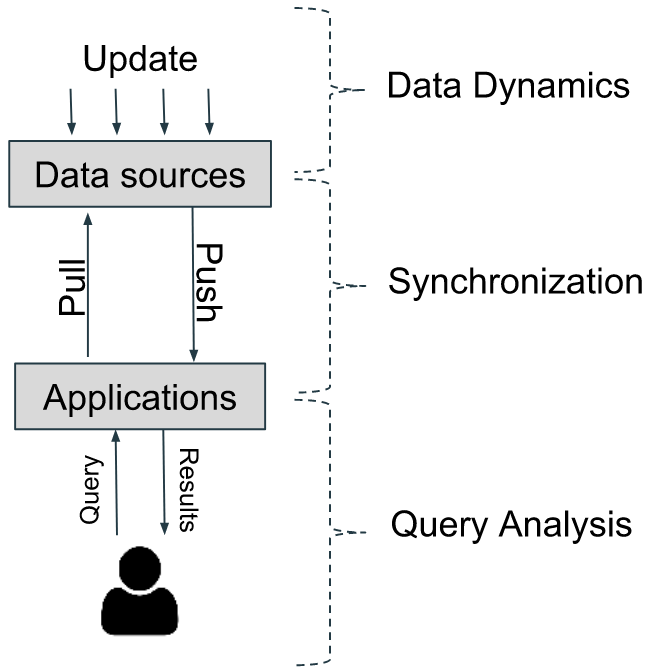
\includegraphics[width=0.9\linewidth]{img/pic}
%	\caption{Typical workflow diagram of a LOD application handling dynamic data.}
%	\label{fig:pic}
%\end{figure}
%
%The survey addresses several \textit{use cases} that could benefit from an understanding of the dynamics of the data and that have been unveiled by several authors. Now we give an introductory summary of the main use cases found in literature~\cite{UmbrichVH10, PopitschH11, KaferUHP12, KaferAUOH13, MeimarisPPGS14}, as well as, the tasks involved in them (although we note that the survey will deepen each task in more depth later):
%
%\textbf{Synchronization:} 
%A application wants to mirror (or copy) the (part of) linked dataset following the ``warehouse'' approaches and must synchronize with the original data source.
%The most common case is to maintain a locally cached LOD index. LinkedData's various centralized search and query methods all rely on local copies of RDF copies collected from the web. If the original data source changes, the replicated index is obsolete and affects the freshness of the results. With a more detailed knowledge of the dynamics of linked data, a centralized engine can, for example, focus on areas that catch up with rapidly changing contributions.
%
%\textbf{Smart Caching:}
%Instead, the ``live querying'' approaches for Linked Data dereference and discover sources on the fly using one or more datasets.However, remote lookups are expensive to execute, thus, it uses a cache that stores local copies of remote data. which must be invalidated when the remote data change. Linking data dynamic knowledge can help to determine the sources that can be cached to save time and resources and the life time of the cached data. An useful example of application can be the smart cache integration of live querying or real-time browsing through Linked Data.
%
%\textbf{Link Maintenance:}
%In LD, publishers embed statements that link local to external resources to use remote data in the local application context. An important point for applications that rely on these links is that links can change, resources can be lost or moved, and new resources can be useful link targets. If the representation of these remote resources changes or becomes unavailable at a particular URI, the application must be notified to keep these links valid. Knowledge of dynamics can help publishers determine how often a linkset needs to be updated based on the target domain or link type.
%
%\textbf{Vocabulary Evolution and Versioning:}
%A specific LOD dataset contains a set of resources, such as clases and properties, that belongs for a particular vocabulary. The definition and structure of the ontologies and vocabularies may change.  changes related with vocabulary terms can affect the interpretation of the remote datasets. So, as vocabulary changes (evolves), there should be some support for spreading vocabulary/ontology changes to the dataset. You must update the dataset to accommodate with new version the vocabulary.
%Learning and understanding the dynamics of vocabularies may inspire and suggest better methodologies for versioning.
%
%\textbf{Hybrid architectures: }
%An important choice for systems that process large amounts of data is to decide between the pre-processing overhead vs the runtime-processing overhead. An application could obtain more benefits in pre-processing (for example, caching, local indexing, reasoning materialization, etc.) of the more static data and leaving the runtime-processing for more dynamic data. In a hybrid architecture, data dynamics information can help decide the most appropriate methods for the data considering that a complex query could contain both. For example, you could decompose a query and answer the static part using the cache and invoke live querying only for the most dynamic part.
%
%\textbf{Change Verification:}
%Many datasets evolve collaboratively in order to keep the information contained as current as possible. While most of the changes that occur in a dataset are correct, erroneous changes also occur due to vandalism or carelessness. Therefore, change verification is required to ensure the quality of the information stored. But manual changes verification is an intensive task. The knowledge of certain evolutionary patterns within the data could help to automatically determine whether the incoming changes are correct or not.
%
%The previous use cases require a technical infrastructure composed mainly of the following components~\cite{UmbrichVH10, PopitschH11}:
%
%\begin{itemize}
%
%\item A \textbf{Change Detection Methods} is an algorithm that is able to extract the differences between different versions of a linked dataset. These algorithms detect the changes taking into account a granularity level (e.g. RDF statements, RDF resources, etc.), a complexity level ( e.g. simples changes or compound changes), and also try to discover these changes in an unambiguous and deterministic way.
%
%\item A \textbf{Change Description Vocabulary} allows you to represent change information readable and understandable by a machine about what and how a certain resource has changed in a dataset.
%
%\item A \textbf{Dynamic Description Vocabulary} can express meta-information about the dynamics of the dataset at different granularity level (e.g. change frequency, change dimension, last update, etc.)
%
%\item A \textbf{Communication Mechanism} also known as notification protocols include the channels to propagate detected changes to consumer based on different initialization policies (e.g. push-based and pull-based)
%
%\item In the absence of mechanisms to propagate changes, the \textbf{Discovery Mechanism} allows applications to discover when changes occur.
%
%\end{itemize}

\subsection{Survey Methodology}\label{Methodology}

This systematic review was carried out following a fusion of the methodologies proposed in ~\cite{keele07, snyder19}. Next, we will present the main methodological decisions included in the review protocol, such as: the research questions we intended to answer, the selection criteria used to determine which studies are included or excluded from a the review, strategy that used to look for primary studies, including search terms and resources to be searched. To reduce the possibilities of reviewer bias, the study was conducted by 3 reviewers from 2 different institutions and we applied some polities for enrich the primary studies based on references to ensure the completeness~\cite{Wohlin14}. 

An overview of our search methodology including the number of retrieved articles at each step is shown in Figure~\ref{fig:methodology} and described in detail below.


\begin{figure*}[h]
	\centering
	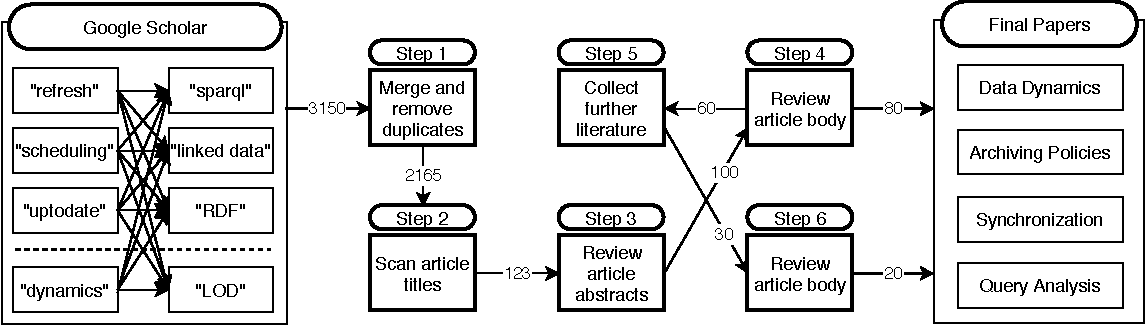
\includegraphics[scale=0.8]{img/methodology.pdf}
	\caption{Number of articles retrieved during literature review.}
	\label{fig:methodology}
\end{figure*}

\subsubsection{Research Question}\label{Question}

The goal of this review is to analyze existing methodologies to consume of Dynamic Linked Open Data. To reach this purpose, we attempt to answers the following research questions: 

\begin{itemize}

\item What methods or models exist to allow applications to consume dynamic linked data? 

\item How data dynamics impact on linked open data consumption models?

\end{itemize}

%\textbf{Complementary Research Questions}

However, apart from these questions related to the technological stack of the consumption of dynamic linked data and more towards a point of view of web science, we are interested in those works that study the intrinsic dynamics of the data web answering some empirical questions related with the change degree and frequency, such as the following:

\begin{itemize}

\item \textbf{Change frequency:} Can we model change frequency of resources and thus predict future changes?

\item \textbf{Change patterns:} Can we mine patterns that help to group by change behavior?

\item \textbf{Degree of change:} How can we quantify how much a resource change?

\item \textbf{Lifespan:} How can we estimate the time-to-live of Linked Data resources?

\item \textbf{Schema evolution:} How dynamics are the schema used in Linked Datasets?

\item \textbf{Structural changes:} Do we observe any changes in the structure of the network formed by links?

\end{itemize}

\subsubsection{Inclusion and Exclusion Criteria}\label{Criteria}

Based on the previous discussion, this survey includes papers that are:

\begin{itemize}

\item focused on the dynamicity of LOD.

\item focused on the synchronization policies used on LOD.

\item focused on query caching/refreshing on LOD.

\item published in English.

\item were peer-reviewed and published.

\end{itemize}

\subsubsection{Search Strategy}\label{Search}

Taking into account our research questions and eligibility criteria, we define two sets of keyphrases. In the first group of we include terms related to evolution or its consequences (e.g. "dynamics", "freshness", "refresh") and in the second group, terms related to the Semantic Web datasets (e.g. "linked data", "SPARQL", "knowledge graphs"). Then the search terms finally used were the product of concatenating the keyphrases from both sets (e.g. "dynamic linked data", "refresh SPARQL"). These groups of keyphrases were enriched iteratively evaluating the adequacy of the most relevant results found and synonyms extracted from the terminology used in some relevant results. Table~\ref{tab:terms} lists the keyphrases used to search for documents.

%\textbf{Search Terms}\label{Terms}

\begin{table}[]
	\centering
	\caption{Keyphrases used to search for primary candidate papers. DY list Keyphrases relating to Dynamics; SW lists Keyphrases relating to the Semantic Web.}
	\label{tab:terms}
	\begin{tabular}{ll} 
		\hline
		type & keyphrases  \\ \hline
		DY    & "refresh"
		"scheduling"
		"uptodate" \\ &
		"cache"
		"change"
		"dynamics" \\ &
		"evolving"
		"fresh"
		"freshness"            \\ \hline
		SW    & "knowledge graphs"
		"linked data" \\ &
		"linked $\cup$ open $\cup$ data"
		"linked open data" \\ &
		"LOD"
		"RDF"
		"sparql"           \\ \hline
	\end{tabular}
\end{table}

%\textbf{Resources}\label{Resources}

Our search strategy consists of 6 phases until the final articles are obtained. In the first phase, we search on Google Scholar using our search terms, merging and removing duplicates from the lists of candidate documents; In the second phase, we made a limited filter by scanning the titles of the articles based on our inclusion and exclusion criteria; In the third phase, we apply a slightly deeper filter by reviewing the abstracts of the articles; in the fourth phase, we filter by the body relevance of the article; In the fifth phase, we expand our set of relevant works including those works referred into the related work, also the works citing the most relevant documents, and also documents written by the most prominent authors; finally, in the sixth phase, these last documents incorporated in the expansion phase are filtered by the body relevance of the article. Figure~\ref{fig:methodology} presents the number of documents considered for each phase of the methodology.

\section{Data Dynamics}\label{Data}

By analyzing some of the most used LOD datasets we can see a clear trend in growth expressed for example in the size, but in this Section, we are interested in the dynamics of that evolution. To query continuously evolving linked datasets, it is useful to understand how datasets (or parts of them) evolve, and how this evolution is related to the data itself, to measure, analyze, and predict data evolution.

Being able to understand and characterize change is important for many practical reasons. When applications locally store descriptions that originate from various remote datasets, awareness of the changes that such descriptions undergo at their origin allows for timely updates, and hence delivering services based on fresh information. Also, an understanding of a dataset's pace of change can inform a decision as to whether an application will cache its content locally, or remotely query it on the fly~\cite{UmbrichKHP12, ekawUmbrichKHP12}.

Given its importance, not a few authors have been concerned with studying the data dynamics with the hope put in the hypothesis that it is possible to predict certain events from observing the previous ones and inferring semantic and context rules. However, on the way to understanding the dynamics they make decisions such as the choice of the dataset, the definition of dynamics and the selection of a methodology to follow.

With respect to the choice of the dataset, it faces the determination of domain, size, completeness, veracity and availability of historical information. With respect to the definition of dynamics, everyone agrees that it is a function of the changes and time, and that is where the distinctions begin between objects to observe the changes (for example, statements, entities, schema, domain, etc.) and the discretization of the time or frequency to observation of changes (for example, hourly, daily, weekly, etc.). For the determination of the methodology, there are variations in the methods used, nevertheless, we distinguish the presence of qualitative and quantitative approaches. Qualitative approaches attempt to detect changes at different levels of complexity according to their definition of dynamics while quantitative approaches attempt to measure change and dynamicity using math functions.

Hereinafter, we explain each of these edges in detail, we describe the main approaches to detect change at certain granularity levels and to perform complex analysis to capture patterns and metrics that allow for characterizing, measuring, and understanding the dynamics of a dataset. At the end, with a general discussion of the achievements and open questions.

As we mention before, the standard approach to represent data published as LD is RDF. It is a graph-structured model based on three disjoint sets of terms: IRIs (\textbf{I}), literals (\textbf{L}), and blank nodes (\textbf{B}). The information is organized into triples $(s,p,o) \in$ \textbf{I} $\cup$ \textbf{B} $\times$ \textbf{I} $\times$ \textbf{I} $\cup$ \textbf{B} $\cup$ \textbf{L}, where $s$ is called subject, $p$ is called predicate, and $o$ is called object. 

\subsection{Versioned Datasets}\label{Datasets}

To understand the dynamics of a data source, information about the historical evolution of that data source is needed, but is rarely accessible. For research on how LD data sources change over time it is desirable to be cross-domain, contiguous, frequent and real-world data, also large-scale, diverse and dynamic. We show what that means:

\begin{itemize}
	
\item \textbf{cross-domain:} capturing a wide selection of Linked Data domains;
\item \textbf{contiguous:} access to consecutive snapshots without holes;
\item \textbf{frequent:} short time between snapshots;
\item \textbf{real-world:} not synthetic data; 
\item \textbf{large-scale:} large number of elements;
\item \textbf{diverse:} suitable for studying for a wide range of applications;
\item \textbf{dynamic:} large changes between versions.

\end{itemize}

We found that there are not many linked versioned datasets with all of these features. For this reason, a number of datasets have been developed and used for research on how LD data sources change over time. 

Umbrich et al.~\cite{UmbrichHHPD10} created a small one consisting of 24 weekly snapshots of RDF Web data used to analyze changes in documents. However, the recovery strategy allowed incomplete changes history for some documents. It is wished monitor the same objects in each version.

The better enforce found was DyLDO, which have been created especially for this purpose\footnote{http://km.aifb.kit.edu/projects/dyldo/data/} and it is used in several studies. It has been created monitoring a fixed set of Linked Data documents (and their neighborhood) on a weekly basis~\cite{KaferUHP12, KaferAUOH13}. As of march 3rd, 2020, it is composed of 399 weekly snapshots corresponding to a period from May 6, 2012 to March 1st, 2020 (both inclusive). Furthermore, the DyLDO dataset contains samples of various well known and large LOD sources, e.g., dbpedia.com, musicbrainz.com, and bbc.co.uk, as well as less commonly known ones, e.g., advogato.org, statistics.data.gov.uk, and uefa.status.net. Using the weekly crawls obtained from the DyLDO dataset, one can only analyze changes occurring between consecutive weeks (e.g., daily changes cannot be considered).

Some of the datasets that are used, some of them  (), while others are datasets that have naturally evolved and where it is possible to access historical changes (Wikidata, DBpedia, etc.). There are also tools that allow for building this historical data (Multicrawler, LDSpider).

Other datasets used, correspond to cross-domain Knowledge Graphs (KG) that have naturally evolved and where it is possible to access historical changes, such as Wikidata and DBpedia. Wikidata~\cite{VrandecicK14} is a large, open cross-domain KG started in October 2012 hosted by the Wikimedia Foundation and it is used by Wikimedia projects, such as Wikipedia. It contains structured information and it is maintained collaboratively by volunteer editors who generate continuous changes. Furthermore, due to the shutdown of Freebase\footnote{http://www.freebase.com}, a popular Knowledge Graph run by Google, data in Freebase have been migrated into Wikidata. Thus, Wikidata is expected to be used in many applications. It is possible to obtain the snapshots from the Wikidata RDF exports\footnote{https://dumps.wikimedia.org/wikidatawiki/entities/} on a weekly basis. 

DBpedia, on the other hand, is a project whose objective is to extract structured content from the information created in the Wikipedia project. Historical information is available \footnote{https://wiki.dbpedia.org/develop/datasets}. However, new releases require manual effort and therefore are not very up to date. DBpedia Live is a DBpedia-based project that processes the hundreds of editions per minute that are generated in wikipedia to provide a constant stream of updates for DBpedia. 

Another alternative is to use crawling software, such as LDSpider~\cite{IseleUBH10} or the MultiCrawler~\cite{HarthUD06} framework to crawl from an initial list of URLs. This produces quad data obtained from dereferencing the seed URIs. The quads contain the triples from the download, with the fourth context position indicating the URI of the information resource from which the triple was downloaded (i.e. the source of the triple).

The last option is to use synthetic data~\cite {MeimarisP16}, which is not useful to study dynamics patterns but to evaluate tools involved such as change detection and archiving.

\subsection{Granularity Levels}\label{Granularity}

When considering a set of LOD sources, undoubtedly some of them change more or less often than others~\cite{KaferAUOH13, DividinoGSG14}. For example, it is not likely that in a short interval of time each source of LOD will change, so it is not necessary to obtain fresh data from static sources. However, when data from a source changes, an update is required. Consequently, some sources must be refreshed at shorter or longer time intervals. This implies that each source of LOD can be assigned a different update importance, which is based on its change behavior. Similarly, within the sources, we may observe different change behavior from different points of view or granularity levels, such as changes involving concepts, properties, or triples.

In more detail, we found works analyzing change behavior at the following levels:
\begin{itemize}
	\item \textbf{d} \textit{Dataset}: the document (RDF Graph) changed;
	\item \textbf{r} \textit{Resource}: the resource (URI) changed;
	\item \textbf{s} \textit{Statement}: the statement (RDF triple) was deleted or added;
	\item \textbf{e} \textit{Entity}: the description of a resource (properties) changed;
	\item \textbf{sh} \textit{Schema}: the property and classes changed;
	\item \textbf{q} \textit{Query result}: the result of specific query changed;
	\item \textbf{D} \textit{Domain}: the document of specific domain (PLD) changed.
\end{itemize}

The works surveyed declare the level of granularity to study dataset evolution. Some approaches are general and do not depend on the object to be studied. The authors agree with the definitions at most levels, but in the case of entity and scheme, there are some variations.

With respect to entity, some works consider an entity's description as the set of triples containing that entity as subject~\cite{UmbrichKL10, NishiokaS15, NishiokaS16, GonzalezH18, DividinoSGG13} and others also consider the set of triples containing $e$ as an object~\cite{UmbrichHHPD10, NishiokaS16}.

In the case of the scheme, some authors study the evolution of the schema taking into account the independent terms used as predicates or classes~\cite{KaferAUOH13, KaferWA17}, others~\cite{DividinoSGG13, GonzalezH18} use the signature of the scheme of documents involving predicates and classes using the concept of $Characteristic$ $Sets$ proposed by Neumann and Moerkotte~\cite{NeumannM11} or changes in their use $Mapping$ $Sets$~\cite{DividinoSGG13}.

\subsection{Change Metrics}\label{Detection}

To understand the dynamics of the datasets, one of the approaches followed is quantitative. For this, it is necessary to define a measure to quantify the changes that have occurred between two versions of an object.

In the literature, several change metrics have been proposed to analyze RDF data in LOD~\cite{UmbrichHHPD10, NishiokaS15}. These metrics essentially quantify the changes that occurred in a resource over time. They are denoted as a $distance$ function and they determine the difference (or distance) between two objects. For example, changes between two sets of data can be measured by the number of differences between the set of statements~\cite{DividinoGSG14} (such as additions and eliminations of RDF triples) or simply stating whether they are equal or different in terms of sets (see Equation~\ref{eq:Inequality}) \cite{UmbrichHHPD10}.

To quantify change, some frameworks~\cite{DividinoGSG14, NishiokaS15} use Jaccard (see Equation~\ref{eq:Jaccard}) for datasets and resources represented as sets, others~\cite{NishiokaS16} use Cosine (see Equation~\ref{eq:Cosine}) or Euclidean distance (see Equation~\ref{eq:Euclidean}) for resources represented as vectors.

\begin{equation}
\label{eq:Inequality}
\delta_{Inequality}(X_1, X_2) = 
\begin{cases} 
0 & X_1 = X_2 \\
1 & otherwise 
\end{cases}
\end{equation}

\begin{equation}
\label{eq:Jaccard}
\delta_{Jaccard}(X_1, X_2) = 1-\frac{|X_1 \cap X_2|}{|X_1 \cup X_2|}
\end{equation}

\begin{equation}
\label{eq:Cosine}
\delta_{Cosine}(R_1, R_2) = 1-\frac{R_1 \cdot R_2}{||R_1|| \cdot ||R_2||}
\end{equation}

\begin{equation}
\label{eq:Euclidean}
\delta_{Euclidean}(R_1, R_2) = \sqrt{\sum_{i=1}^n (R_{1i} - R_{2i})^2}
\end{equation}

Equation~\ref{eq:Inequality} and Equation~\ref{eq:Jaccard} consider the objects to be compared as sets; for example, a resource or a dataset may be described by a set of triples. Equation~\ref{eq:Cosine} and Equation~\ref{eq:Euclidean} are based on widely used metrics and assume the input $R_i$ as vectors of $R_{ij}$ values.

It is desired to compare RDF content, not document syntax; thus, the comparison is complicated by the presence of blank nodes. For example, to check if the content of an RDF graph with blank nodes has changed over time it is necessary to check graph isomorphism between RDF graphs. This is difficult, because of the size of the graphs and the complexity of the task, so some works filter out triples that contain a blank node from the snapshots~\cite{NishiokaS18, KaferAUOH13} while others detect isomorphisms among RDF graphs from different snapshots and replace the blank nodes by URIs~\cite{UmbrichHHPD10}, using hash-based skolemization as per the approach described by Hogan in~\cite{Hogan15}.

The number of changes observed in the two snapshots does not reflect the entire history of changes that occurred between them. To quantify the evolution of a dataset it is necessary to take into consideration the changes occurring over a period of time. Dividino et al.~\cite{DividinoGSG14} define dynamics as an aggregation of changes (see Equation~\ref{eq:dyn}), built on top of contemporary change metrics $\delta$ (see Equation~\ref{eq:Inequality}-\ref{eq:Euclidean}). They understand a period of time as a continuous time interval beginning at an initial point in time $t_1$ up to a final one $t_n$ and defined the dynamics of a dataset as the integration of its change rate over time (see Figure~\ref{fig:d1}). Due to this time-dependence, a measure for dynamics should capture the frequency, degree, and regularity of the data changes. However, also the change rate function is not explicitly known, and cannot be used for the computation, i.e., it is not possible to determine the change rate of a dataset for a given point in time. Thus, their idea was to use an approximation based on discrete points in time and the changes between the datasets at these times (see Equation~\ref{eq:dyn} and Figure~\ref{fig:d2}).

\begin{figure}[h]
	\centering
	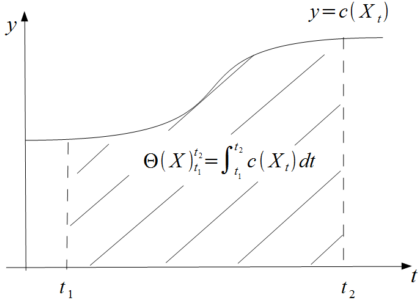
\includegraphics[scale=0.4]{img/d1.png}
	\caption{The dynamics as an integration of a continuous change function over time~\cite{DividinoGSG14}.}
	\label{fig:d1}
\end{figure}

\begin{equation}
\label{eq:dyn}
\Theta(X)^{t_n}_{t_1} = \sum_{i = 2}^{n} \delta_{metric}(X_{t_i}, X_{t_{i-1}})
\end{equation}

\begin{figure}[h]
	\centering
	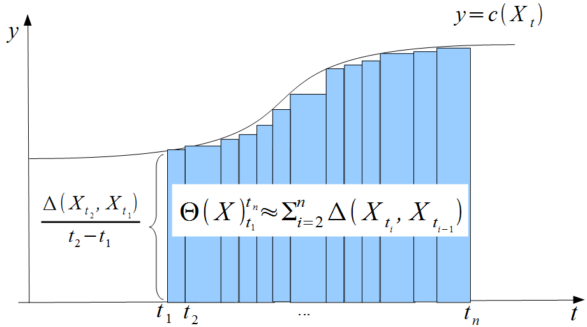
\includegraphics[scale=0.3]{img/d2.png}
	\caption{The dynamics as aggregation of $\delta_{metric}$~\cite{DividinoGSG14}.}
	\label{fig:d2}
\end{figure}

However, for most applications, the changes tend to be less important as time goes by, for example, if a dataset used to change a lot but no longer does, it may be necessary to adapt its index update strategy. For this purpose, some frameworks~\cite{DividinoGSG14, KnuthHS16} extend this notion (see Equation~\ref{eq:dyn:decay}) incorporating a decay function within the dynamics computation to differentiate the changes depending on when they occurred in the observed time interval using the exponential function (see Equation~\ref{eq:decay}) as an aging factor ($\lambda$).

\begin{equation}
\label{eq:decay}
f(i) = e^{-\lambda (n-i)}
\end{equation}

\begin{equation}
\label{eq:dyn:decay}
\Theta_{decay}(X)^{n}_{1} = \sum_{i = 2}^{n} f(i) \delta_{metrics}(X_{i}, X_{i-1})
\end{equation}

\subsection{Change Detection}

In the qualitative approach, rather than measuring how much the datasets have changed, we care to understand their evolution by finding and analyzing the differences between different versions of the data. 

The information of how a certain data unit has changed is typically expressed by operations, $add$ and $deleted$ being the atomic (low-level)~\cite{UmbrichHHPD10} ones. From a set of atomic operations, one can derive so-called compound changes or even higher-level changes~\cite{PapavasileiouFFKC13}.

Simple changes are intended to capture fine granularity types of evolution and must be defined to meet the formal requirements of completeness and unambiguity to ensure a correct detection process~\cite{PapavasileiouFFKC13}. 

Managing changes poses several research problems, including the problem of detecting the changes ($delta$) between versions of the same dataset. This approach is followed to understand what is changing and what transformations are happening in the data.

A change detection tool is essentially based on a language of changes, which describes the meaning of the different change operations that the underlying algorithm understands and detects. An important requirement for change detection tools is their ability to produce deltas that can be interpreted both by humans and machines. In its simplest form, a language of changes consists of only two low-level~\cite{UmbrichHHPD10}, \cite{KaferAUOH13} operations, $Add(x)$ and $Delete(x)$, which determine individual constructs that were added or deleted. 

The low-level change detection of a document or entity between two snapshots $t$, $t^\prime$ is not a complex task so long as the statements of the resource do not contain blank nodes. Most of the works found~\cite{UmbrichHHPD10} \cite{UmbrichKL10} used straightforward approach based on a merge-sort scan over the snapshots as follows:

\begin{enumerate}
	\item sort all relevant statements for the change detection of a document or entity by their syntactic natural order (subject-predicate-object);
	\item perform a pairwise comparison of the statements by scanning two snapshots in linear time;
	\item trigger a detection of the change (either w.r.t. a document or entity) as soon as the order of the statements differs between two snapshots (e.g., new statements were added or removed).
\end{enumerate}

The representation of changes in the triplet level leads to a syntactic delta~\cite{ZeginisTC11}, which does not adequately capture the intention behind a change and generates results that are not intuitive enough for the human user. So, a high-level language is preferable to a low-level one in terms of human interpretability, because it is more intuitive, concise, and closer to human intuition, thereby capturing the semantics of a change more accurately.

Some works proposed methods~\cite{PapavasileiouFFKC13}, \cite{RoussakisCSFS15} to achieve high-level changes from low-level ones. They understand high-level changes as real-world actions, which often require several low-level changes.

High-level change operations describe more complex semantic changes~\cite{RoussakisCSFS15} that are related to several low-level changes. However, the detection of high-level change operations involves a series of problems related to the machine-interpretability. For this reason, detecting them becomes more difficult. Then, they defined a high-level and low-complexity type of changes called simple changes. Figure~\ref{fig:cd} shows an example of the different types of complexity of the changes that can be extracted from two versions of an RDF dataset. For example, the incorporation of a player to a soccer team, could involve the addition of several triples with player data and the association to the team.

\begin{figure*}[h]
	\centering
	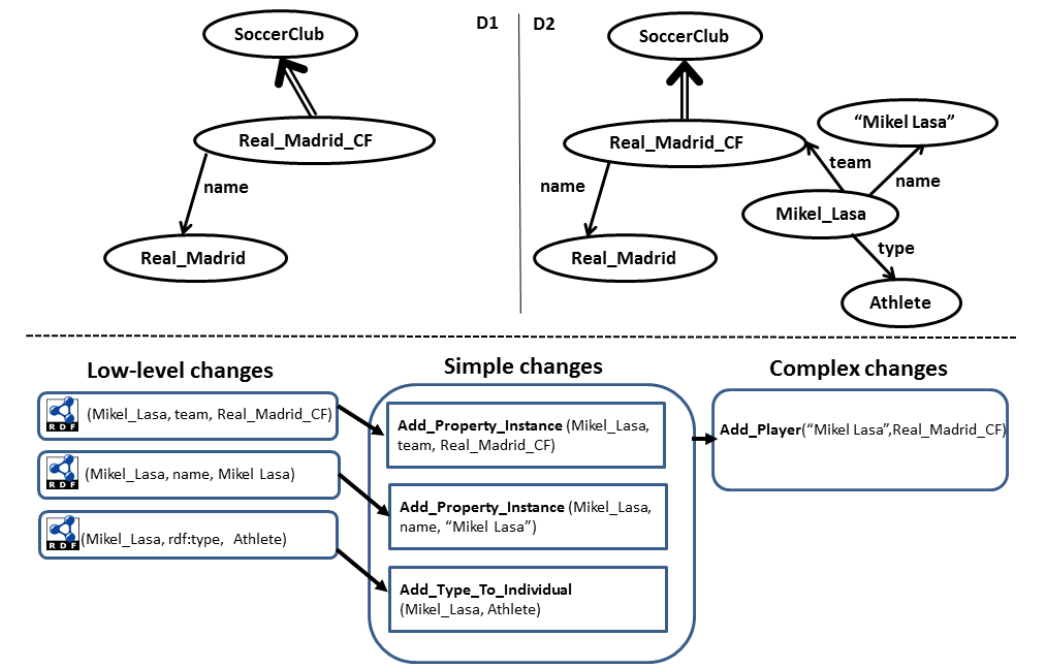
\includegraphics[scale=0.3]{img/cd.png}
	\caption{From de snapshots to the changes~\cite{RoussakisCSFS15}.}
	\label{fig:cd}
\end{figure*}

\subsection{Change Descriptions}\label{Descriptions}
~\cite{PopitschHR10,UmbrichVH10,SandersonS12,MeimarisP16}

When dealing with dataset dynamics, we need a way to describe how dynamic a dataset is, and what has changed. A data consumer can then understand what changed and when further changes can be expected. The descriptions should be machine-readable and should use the same set of RDF vocabularies. However, there is no consensus on the appropriate set of vocabularies to use to represent the evolution of a dataset. 

The Dataset Dynamics group\footnote{https://www.w3.org/wiki/DatasetDynamics} lists a number of vocabularies for representing dataset changesets and updates, such as The Talis Changeset vocabulary\footnote{http://vocab.org/changeset/schema.html}, Delta vocabulary\footnote{https://www.w3.org/2004/delta} and Triplify Update vocabulary\footnote{http://triplify.org/vocabulary/update}. In a more recent work Ellefi et al.~\cite{Ellefi17} survey other proposals, such as the Revision Management Ontology (RMO)~\cite{GraubeHU14} and the Dataset Dynamics (DaDy) vocabulary\footnote{http://vocab.deri.ie/dady}.

To capture specific characteristics and observations related to dynamics and evolution, Table~\ref{tab:vocab} show we some vocabularies, format and ontologies used. We have classified the vocabularies according to their description capacity. We have classified according to their description capacity. The first, Change, addresses the description of the change at a certain level and the second, Dynamics, allows the editors to characterize the change with a temporal dimension, e.g., frequency.

% Table generated by Excel2LaTeX from sheet 'Hoja2'
\begin{table}[htbp]
	\centering
	\caption{Summary of description proposals.}
	\begin{tabular}{lcc}
		\hline
		Works & Change & Dynamics \\ \hline
		Delta \cite{Berners04} & \cmark   & \\
		Talis Changesets \cite{TunnicliffeD09} & \cmark   & \\		
		OWL 2 \cite{PalmaHCG08} & \cmark   &  \\
		CHAO \cite{NoyCLM06} & \cmark   & \\	
		Semantic SiteMaps \cite{CyganiakSDDT08} &    & \cmark \\
		Triplify Update \cite{AuerDLHA09} & \cmark   & \\	
		Dady \cite{Dady10} &    & \cmark \\
		Graph Update Ontology (GUO)\footnotemark	 & \cmark   &  \\
		DSNotify Eventset \cite{PopitschH11} & \cmark   & \\		
		RMO \cite{GraubeHU14} & \cmark   &  \\	
		Ontology of Changes \cite{RoussakisCSFS15} & \cmark   &  \\
		RDF Patch\footnotemark  & \cmark   &  \\ 
		$O^{DE}$ \cite{PernelleSMT16} & \cmark   &  \\ 
		\hline
	\end{tabular}%
	\label{tab:vocab}%
\end{table}%

\footnotetext{http://purl.org/hpi/guo\# }
\footnotetext{http://afs.github.io/rdf-patch/ }


\subsection{Summary}\label{Summary1}

Table~\ref{tab:dyn} provides an overview of the techniques (previously discussed) used by the systems to address the study of datasets dynamics. As you can see, in this section we include those documents that study different datasets from the temporal perspective, we include, the datasets and the unit they study; the metric used in case of quantitative analyzes, or the type of change detected and represented. Based on these criteria, we have excluded those works with important theoretical contributions to the dynamics techniques but that do not have a specific analysis over a concrete dataset.

In this table, \textbf{Year} corresponds to the year of publication, \textbf{Granularity} specifies the basic unit of study, for example statements or entities, which are the most used, \textbf{Datasets} reference the data sets used in the study. For quantitative analyzes, the metrics used under the \textbf{Metric} column are shown, while for the qualitative ones the \textbf{Detection} column is provided with the different types of events detected and in some cases represented using a format or vocabulary for their \textbf{Description}.

% Table generated by Excel2LaTeX from sheet 'Hoja1'
\begin{table*}[]
	\centering
	\caption{Overview of data dynamics approaches.}
	\label{tab:dyn}
	\begin{tabular}{lrlllcr}
		\hline
		Works & \multicolumn{1}{l}{Year} & Granularity & Metric  & Detection & Description  & Datasets \\ \hline
		Umbrich et al. \cite{UmbrichHHPD10} & 2010 & d, e, D &  & low (c, r, u)   &    & MultiCrawler \\
		Popitsch et al. \cite{PopitschHR10,PopitschH10,PopitschH11} & 2010 & s, r & & low (c, r, u, m) & DSNotify Eventset & DBpedia, IIMB\footnotemark \\
		Umbrich et al. \cite{UmbrichKL10} & 2010 & r &  & low (c, r, u)  & & LDSpider \\
		K{\"{a}}fer et al. \cite{KaferAUOH13} & 2013 & d, s, sh, D &  & low (c, r)   &  & LDSpider \\
		Dividino et al. \cite{DividinoSGG13} & 2013 & sh, e &  & low (c, r, u(e))  &   & DyLDO \\
		Papavasileiou et al. \cite{PapavasileiouFFKC13} & 2013 & s &  & high &    & CIDOC, GO, MO \\
		Dividino et al. \cite{DividinoGSG14} & 2014 & s & Jaccard &  &  & DyLDO \\
		Nishioka and Scherp \cite{NishiokaS15} & 2015 & e, D & Jaccard &  & & DyLDO \\
		Roussakis et al. \cite{RoussakisCSFS15,StefanidisFCR16} & 2015 & s &  & high (s, c) & Ontology of Changes  & DBpedia \\
		Pernelle et al. \cite{PernelleSMT16} & 2016 & s &  & low (c, r) & Ontology $O^{DE}$   & DBpedia, FMA, EFO \\
		Nishioka and Scherp \cite{NishiokaS16} & 2016 & e, D & Cosine, Euclidean &  &   & DyLDO \\  
		Knuth et al. \cite{KnuthHS16} & 2016 & q & Inequality &  &  & DBpedia live \\  
		K{\"{a}}fer et al. \cite{KaferWA17} & 2017 & d, s, sh &  & low (c, r)  & DyLDO  Model  & DyLDO \\
		Akhtar et al. \cite{AkhtarAL17} & 2017 & q & Inequality &  &   & DyLDO \\ 
		Gonz\'{a}lez and Hogan \cite{GonzalezH18} & 2018 & sh, e &  & high  &  & Wikidata \\
		Nishioka and Scherp \cite{NishiokaS18} & 2018 & s &  & low (c, r)  &  & Wikidata \\
		Moya and Hogan \cite{LoustaunauH19} & 2019 & q & $Jaccard^*$ &  &  & Wikidata \\
		\hline
	\end{tabular}%
\end{table*}%

\footnotetext{ISLab Instance Matching Benchmark~\cite{FerraraLMV08} }

	\begin{description}
	\item[Umbrich et al. \cite{UmbrichHHPD10}]  analyzed 24 data dumps collected by weekly snapshots of the LOD cloud to understand how the LOD datasets change and what sensible measures there are to accommodate dataset dynamics. They proposed a framework to detect and measure dataset dynamics detecting change at Document and Entity levels, and they presented statistics on the detection of low-level changes that effectively verified the dynamism of the entities. They also showed that it is not feasible to use HTTP headers to detect changes due to the lack of this information. In addition, they could not verify that the frequency of the change followed the Poisson Process change model, because they had an incomplete change history. Although the datasets studied were not very large, the period studied was brief and the authors did not perform a very extensive analysis of patterns of change, this work constitutes a general scheme that can be reused.
	
	\item[Umbrich et al. \cite{UmbrichKL10}] set out to understand what correlations between resources and their dynamics can be identified using methods from Data Mining (DM), Machine Learning (ML), and graph analysis. They propose a framework to categorize LOD resources with respect to their dynamics behavior, defining dynamics by features, monitoring four different events (appears, disappear, change, and no change) and then they used k-means clustering. Although their experiments use a small history of changes, the main value of their work was their motivation and initial ideas to study the dataset dynamics of the LOD Web using ML and DM approaches.
	
	\item[K{\"{a}}fer et al. \cite{KaferAUOH13}] investigated how stable documents were over time and what kinds of changes were most frequently encountered. They did a comprehensive analysis of various monitoring, detecting, and counting changes over LOD sources in 29 consecutive weeks. They contributed mainly in two important ways, building an important dataset (DyLDO) and presenting many statistics about stability, lifespan, frequency, and types of change at different granularity levels. They also found important patterns like that dynamicity tended to follow certain predictive patterns for Pay Level Domains (PLD), that many documents did not change over long periods, and found that many domains were considered static (and thus are candidates for long-term caching). They also identified particular predicates whose triples should not be cached due to high rates of updates.
	
	\item[Dividino et al. \cite{DividinoSGG13}] studied how dynamic is the use of the vocabularies in the cloud. They investigated the dynamics of the schema w.r.t. its usage in a more high-level way: the URI representing some entity, is described by a set of properties and a set of types applying the notion of Extended Characteristic Sets (ECS). They found that even though the vocabulary itself does not change very much, its use does change. Their work offered an early investigation of different metrics applied to schema information and provided a quantitative analysis on the schema information of the DyLDO dataset even though they do not identify patterns of schema changes to use as indicators for predictions.
	
	\item[Papavasileiou et al. \cite{PapavasileiouFFKC13}] studied the problem of detecting the changes (delta) between versions of the same KG and proposed a change language that can describe unambiguously any possible change encountered in curated KGs expressed in RDF(S), and that can be efficiently and deterministically detected in an automated way.
	
	\item[Dividino et al. \cite{DividinoGSG14}] proposed a function to measure the dynamics of a LOD dataset, which is defined as the aggregation of absolute, infinitesimal changes, provided by traditional change metrics. They then investigated the dynamic quantification of selected LOD resources from DyLDO dataset.
	
	\item[Roussakis et al. \cite{RoussakisCSFS15}] also proposed a framework that enables identifying, analyzing, and understanding these dynamics allowing persistent representation of the detected changes between versions. They understood this evolution by finding and analyzing the differences (deltas) between datasets based on SPARQL queries. Their Framework also allows for the creation of an ontology that offers a persistent representation of the detected changes in a way that permits easy and efficient navigation among versions, deltas, snapshots, or historical queries.
	
	\item[Nishioka and Scherp \cite{NishiokaS15, NishiokaS16}] investigated how to determine the temporal patterns of entity dynamics on the cloud. For that they measured the degree of changes of entities between two snapshots; they then represented the dynamics of entities as time series to apply k-means++ clustering and find out temporal patterns of entity dynamics. They also investigated which features of entities control patterns of entity dynamics measuring the relation between some features (Type, Predicates, ECS, PLD) and the dynamics of an entity, finding that the entities that share a common PLD are more likely to change together over time and that the entities that have the same type are more likely to change together.
	
	\item[K{\"{a}}fer et al. \cite{KaferWA17}] proposed an RDF model of change descriptions at physical and logical levels. Their model allows for carrying out more comprehensive analyses of dynamic Linked Data in a declarative fashion. They showed the usefulness of their model by repeating analyses of dynamics using SPARQL queries.
	
	
	\item[Gonz\'{a}lez and Hogan \cite{GonzalezH18}]proposed a framework for computing a data-driven schema from large-scale knowledge graphs based on Formal Concept Analysis. They first extract the sets of properties associated with individual entities; these property sets (aka. characteristic sets) are annotated with cardinalities and used to induce a lattice based on set-containment relations. Then one can use this framework to model and predict the dynamic behavior of Knowledge Graphs by computing changes between lattices.
	
	\item[Nishioka and Scherp \cite{NishiokaS18}] developed classifiers for assessing whether changes on a KG were correct by exploiting the features from KG evolution analysis. They analyzed how KGs evolve over time monitoring how useful were some topological features of the KG for change verification.
	
	
\end{description}

\subsection{Open Questions}\label{Open1}

Lorem ipsum dolor sit amet, consectetur adipiscing elit, sed do eiusmod tempor incididunt ut labore et dolore magna aliqua. Ut enim ad minim veniam, quis nostrud exercitation ullamco laboris nisi ut aliquip ex ea commodo consequat. Duis aute irure dolor in reprehenderit in voluptate velit esse cillum dolore eu fugiat nulla pariatur. Excepteur sint occaecat cupidatat non proident, sunt in culpa qui officia deserunt mollit anim id est laborum.

Curabitur pretium tincidunt lacus. Nulla gravida orci a odio. Nullam varius, turpis et commodo pharetra, est eros bibendum elit, nec luctus magna felis sollicitudin mauris. Integer in mauris eu nibh euismod gravida. Duis ac tellus et risus vulputate vehicula. Donec lobortis risus a elit. Etiam tempor. Ut ullamcorper, ligula eu tempor congue, eros est euismod turpis, id tincidunt sapien risus a quam. Maecenas fermentum consequat mi. Donec fermentum. Pellentesque malesuada nulla a mi. Duis sapien sem, aliquet nec, commodo eget, consequat quis, neque. Aliquam faucibus, elit ut dictum aliquet, felis nisl adipiscing sapien, sed malesuada diam lacus eget erat. Cras mollis scelerisque nunc. Nullam arcu. Aliquam consequat. Curabitur augue lorem, dapibus quis, laoreet et, pretium ac, nisi. Aenean magna nisl, mollis quis, molestie eu, feugiat in, orci. In hac habitasse platea dictumst.

\section{Archiving Policies}\label{Archiving}
~\cite{SandersonS12,Papastefanatos13,MeimarisPPGS14}

\subsection{RDF Archives}\label{Archives}
\subsection{Query Types}\label{Types}
\subsection{RDF Archive Benchmarks}\label{Benchmarks}
\subsection{System Summary}\label{System3}
\subsection{Summary}\label{Summary3}
\subsection{Open Questions}\label{Open3}


\section{Synchronization}\label{Index}ls

We have seen in the previous section that the Web of Data is dynamic, that Linked Data sources are updated autonomously and that applications must be aware of those changes. In this section, we will study the works and tools developed to allow applications to synchronize their data with those of the sources. Synchronization allows for timely updating, and hence delivering services based on fresh information.

One approach might be to update the data very frequently. However, due to limitations of the available computational resources (e.g., network bandwidth for fetching data, and computation time) LOD applications may not be able to permanently visit the LOD sources at brief intervals in order to check for changes.

Thus, the research question is: \textit{How to determine the best time at which a relevant data change has occurred?}

Ideally, the consumers want to receive information about the statements that have been added/deleted at a particular time. Notification about the changes offers an efficient way to keep data updated, but this approach is often not the most appropriate. Another way to detect changes is to exploit the HTTP header information provided on the Web, but some works have shown that these data are often not provided or are wrong~\cite{UmbrichHHPD10, DividinoKG14, Kjernsmo15, NeumaierU16}. Therefore, most applications must rather rely on the estimation of changes to provide quality services expressed in terms of response time, data freshness, and completeness.

The estimation of change is a difficult task that several authors have tried to solve. A perfect estimation is not expected, because the evolution of the data approaches the real phenomena, which in many occasions are unpredictable. Figure \ref{fig:syn} shows a history of an example changing data item. On average this item changes half of the time, however the strategy of following the average is not able to capture all the changes and at the same time, it searches for redundant calculations. One can see the difficulty of the task.

\begin{figure}[h]
	\centering
	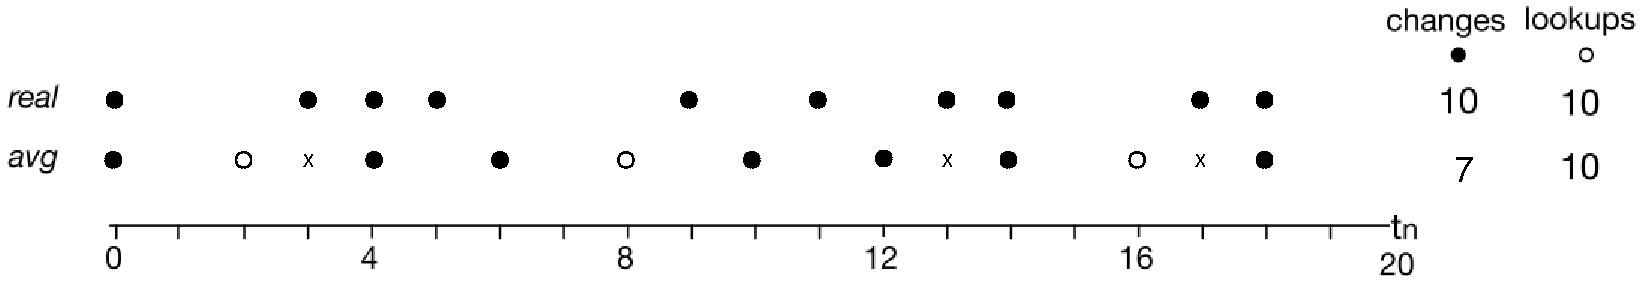
\includegraphics[width=1\linewidth]{img/syn.pdf}
	\caption{Change's history of a data and how average strategy capture or miss those changes.}
	\label{fig:syn}
\end{figure}

In this Section, we classify synchronization methods according to several dimensions characterizing their algorithms, such as (i) whether the synchronization is triggered by the consumer (pull-based) or the source (push-based), (ii) the ability to deterministically recognize the update time, and (iii) the foundation of estimation methods. Based on this classification, we review the methods proposed in the literature to solve the updating problem. Additionally, we compare the surveyed methods with respect to other dimensions, such as resource constraints they consider during the update process, quality achieved, datasets used, and dynamic features they consider.

\subsection{Synchronization Policies}\label{Synchronization}
~\cite{UmbrichHHPD10}

There are two possibilities to collect the change time for a given resource:
\begin{itemize}
	\item push-based approaches for which the data publishers provide change notifications.
	\item pull-based approaches for which one periodically checks if a data source has changed.
\end{itemize}

The push-based approach ensures that updates are reported to clients in a timely manner and is useful for many applications. However, push-based delivery may not be cost effective or feasible in all situations. Some scenarios are well suited to push, for example, a small group of clients who need to be notified of updates in a timely manner. In this case, push-based strategies could eliminate the need for clients to frequently poll servers, thereby reducing server load. However, only data providers can offer an information service based on push and it is not available in most cases. Therefore, applications have to rely on the other, pull-based approach, to collect change information. 

The pull-based monitoring approach has the obvious drawbacks of being more resource consuming than push-based change information. In addition, the monitoring interval influences how accurately one can sample the change times. For instance, the monitoring approach can only detect the last change between two monitoring intervals, even if several changes occurred during two monitoring points.

Table~\ref{tab:syn} lists some work that has been proposed for communication between dataset consumers and publishers.

% Table generated by Excel2LaTeX from sheet 'Hoja2'
\begin{table}[htbp]
	\centering
	\caption{Summary of synchronization mechanism.}
	\begin{tabular}{lcc}
		\hline
		Mechanism & Push & Pull \\ \hline
		SparqlPuSH \cite{PassantM10} & \cmark   & \\
		DSNotify \cite{PopitschH11} &   & \cmark \\
		online services\footnotemark & \cmark   & \\
		PubSubHubbub \cite{Fitzpatrick10} & \cmark   & \\
		Semantic Pingback \cite{TrampFEA10} & \cmark   & \\
		RDFSync \cite{TummarelloMBE07} &   &  \cmark  \\
		rsine \cite{MaderMS14} & \cmark   & \\
		Boca RDF \cite{MissierACDG07} & \cmark   & \\
		Atom \cite{Nottingham05} &    &  \cmark \\
		\hline
	\end{tabular}%
	\label{tab:syn}%
\end{table}%

\footnotetext{http://www.changedetection.com/}

\subsubsection{Change Notifications}\label{Notifications}
~\cite{UmbrichVH10}
Ideally, the consumer wants to be informed about the statements that have been added/removed at a certain time point. The notification about changes offers an efficient way to keep their data updated.

The study of Linked Data notifications is very relevant for a broad range of application domains. Currently, one of the most popular Linked Data notification approach, sparqlPuSH~\cite{PassantM10}, allows users to register a SPARQL query and get updates pushed to the user as new matching triples arrive in an underlying triple store containing relevant data. It relies on SPARQL queries, tracks changes of the result set published as an RSS feed, and broadcasts change notifications via the PubSubHubbub protocol. A more recent work is Resource Subscription and Notification sErvice (rsine)~\cite{MaderMS14}, a framework that notifies subscribers whenever resources are updated, created, or removed. It is comparable to sparqlPuSH, but it is designed to operate on a more general level, not only queries. In contrast to sparqlPuSH, rsine intends to maintain the quality of controlled vocabularies. Boca RDF~\cite{MissierACDG07} provides a change detection sub-system based on Sun’s Java messaging service. Users will get notifications when there is any change in individual RDF statements or the entire graph.

The push scenario assumes that the data provider sends the change notification to the client or to a hub, therefore, the change history will contain the complete set of all change times. While, push-based mechanisms can deal very efficiently with data that changes frequently, on the other hand, these mechanisms must maintain a subscriber list and open connection states that can also cause scalability problems as the number of clients grows. On the other hand, pull-based mechanisms consume more bandwidth resources.\\

\subsubsection{Change Monitoring}\label{Monitoring}
~\cite{UmbrichHHPD10}

%HTTP-metadata Monitoring

Given that the HTTP protocol is recommended by the Linked Data guidelines, the most intuitive way for clients to detect changes would be to exploit the HTTP header information provided on the Web.

The information contained in HTTP response headers offers fields to indicate a change in a document. Using such methods of change detection is more economical in that it avoids the need for content sniffing, but some works~\cite{UmbrichHHPD10, DividinoKG14, Kjernsmo15, NeumaierU16} show that these data are often not provided or are wrong.

Dividino et al.~\cite{DividinoKG14} evaluated the conformance of LOD data source to provide a valid and correct $Last$-$Modified$ HTTP header field, which indicates the date and time at which the resource was last modified. Their experiment shows that overall and on average only 8\% of the resources in the datasets provide correct values for this field. This number is far too low to be of use for any practical application.

Umbrich et al.~\cite{UmbrichHHPD10} verified the use (or lack of) of the $Etag$ and $Last$-$Modified$ field for a corpus of 550K documents and found that 67.95\% did not report either of these two fields. Therefore, it is not feasible to rely on this information to detect changes.

Kjernsmo~\cite{Kjernsmo15} investigated many of the HTTP caching implementations (i.e., LOD servers) and examines the availability and conformance of the HTTP headers that may allow caching. Even on different datasets, the authors conclude that the headers do not reflect the standards compliant lifetimes advertised by servers, and therefore they are not helpful for applications relying on caching.

Neumaier and Umbrich~\cite{NeumaierU16} inspected the HTTP Headers of a total of 3.1 million resources reveals that 66\% of the CKAN, 100\% of the Socrata and 0\% of the OpenDataSoft resources have the $Last$-$Modified$ header field.

To investigate the use of temporal information, Rula et al. ~\cite{RulaPHSM12} ascertained how many of the URIs that identified documents in the 2011 Billion Triple Challenge (BTC) dataset returned date information in the HTTP header. For that, they generated a random sample of 1000 documents (from the context of the quads), and for each document URI in the sample and they perform an HTTP lookup to check the $Last$-$Modified$ header in the HTTP response. They found again that only 95 out of 1000 URIs returned $Last$-$Modified$ headers.  

The Sitemap extension~\cite{CyganiakSDDT08} offers another solution, defining how often data can be re-crawled from a website to get fresh information, but it relies on clients regularly fetching it, not directly solving the synchronization issue. 

\subsubsection{Change Prediction}\label{Prediction}
~\cite{UmbrichHHPD10,BarsottiDD17a,GonzalezH18}

Typically, dataset providers do not offer any mechanism to inform clients about data updates: if the data has changed nor to what extent. Therefore, in this Section, we focus on synchronization strategies that are dataset agnostic, i.e., strategies that do not assume meta-data about what has changed since the last update. Table~\ref{tab:pull} shows surveyed works relating to Pull-Based Synchronization Approaches.\\

\begin{table*}[h]
	\centering
	\caption{Overview of Pull-Based Synchronization Approaches.}
	\label{tab:pull}
	\begin{tabular}{llll} \hline
		Works                                            & Year & Models                          & Datasets          \\ \hline
		Umbrich et al. \cite{UmbrichHHPD10}                & 2010 & Poisson Process                          & MultiCrawler        \\
		Umbrich et al. \cite{UmbrichMP15}                 & 2015 & Adaptive Heuristics, Markov Chains           & Wikipedia          \\
		Dividino et al. \cite{DividinoGS15}                & 2015 & History Metrics     & DyLDO            \\
		Neumaier and Umbrich \cite{NeumaierU16}         & 2016 & Empirical Distribution, Poisson Process, Markov Chains              & CKAN, Socrata, OpenDataSoft \\
		Knuth et al. \cite{KnuthHS16}                   & 2016 & History Metrics, Adaptive Heuristics & DBpedia Live         \\
		Nishioka and Scherp \cite{NishiokaS17}          & 2017 & Machine Learning     & DyLDO            \\
		Akhtar et al. \cite{AkhtarAL17}                  & 2017 & History Metrics                  & DyLDO(DBpedia), LSQ     \\
		Gonz\'{a}lez and Hogan \cite{GonzalezH18}         & 2018 & Machine Learning                         & Wikidata  \\  \hline      
	\end{tabular}
\end{table*}

\textbf{Empirical Distribution}: 

A simple method is to build an Empirical Distribution function based on the intervals between observed changes. An Empirical Distribution function is a distribution function associated with the empirical measure of a sample. This cumulative distribution function is a step function that jumps up by $ \frac{1}{n} $ at each of the $ n $ data points. Its value at any specified index of the measured variable is the fraction of observations of the measured variable that are less than or equal to that at the specified index.

\begin{example}
	\label{ex:ED}
	Based on the following change history (00111000100011000100001), where 0 indicates no change, and 1 a change based on comparing the content at the current point with the content at the previous sampling point. This history results in the intervals (31144145) which one can use as input for an Empirical Distribution.
\end{example}

Neumaier and Umbrich~\cite{NeumaierU16} evaluated this method for estimating freshness in Open Data Portals.\\

\textbf{Poisson Process}:

Cho and Garcia-Molina~\cite{ChoG00} modeled change frequencies of Web documents as Poisson Processes. The Poisson Process is one of the most widely-used counting processes. It is usually used in scenarios where we are counting the occurrences of certain events that appear to happen at a certain rate, but completely at random. For instance, occurrences of fatal auto accidents, arrivals of customers at a service center, telephone calls originating in a region, etc., are usually modeled by a Poisson Process. 

It is believed that a Poisson Process is a good model for changes on the Web of Data too. However, we found no studies showing that the assumption of a Poisson Process also holds for the sources on the Web of Data.

To describe the Poisson-process model, we use $X(t)$ to refer to the number of occurrences of a change in the interval $(0, t]$. Then, a Poisson Process of $rate$ or $frequency$ $\lambda$ has the following property:

For $s \geq 0$ and $t > 0$, the random variable $X(s + t) - X(s)$ has the Poisson probability distribution

\begin{equation}
\label{eq:Poisson}
P\\(X(s + t) - X(s) = k\\) = \frac{(\lambda t)^k}{k!}e^{-\lambda t} for~k=0,1,...
\end{equation}

Umbrich et al.~\cite{UmbrichHHPD10} analyzed whether they can apply this Poisson model to the changes of documents and entities detected on LOD and concluded they cannot accept nor reject the described change model with statistical significance.

Neumaier and Umbrich~\cite{NeumaierU16} followed an improved estimator provided by Cho and Garcia-Molina~\cite{ChoG03} to avoid the effects of incomplete change history. They improved this estimator, because they showed that the estimation is highly biased if the update history is incomplete, i.e., if there are changes to the resource, which are not detected by the sampling. However, in the case of this work, the results were not notably different from those of the traditional Poisson Process.\\

\textbf{Markov Chains}:

Another strategy is to apply the Markov Chains approach to determine the likelihood to observe a change in future considering the past observed changes. 

A Markov chain is a probabilistic process where the probability distribution of the next state depends on the current state only. This is stated in the so-called Markov property: given a present state, the future and past states are independent.

\begin{example}
	Using the change history of Example~\ref{ex:ED}, we can build a state-change matrix by counting the state transitions. Figure~\ref{tab:state1} shows the example considering only the last state of the data to compute the likelihood of the next state. For instance, the value (i = 1, i + 1 = 1) indicates that we observed 3 times that the data changes consecutively in a row and that we observed 5 times a change after a non-change (i = 0, i + 1 = 1). We use this information to determine how likely it is that the data changes in the next time: For instance, considering our example table: $P(1|0) = \frac{5}{15} = 0.33$. Figure~\ref{tab:state2} considers the last two change states of the data to compute the likelihood of the next change state.
\end{example}    

\begin{figure}[h]
	\begin{minipage}[b]{0.45\linewidth}
		\begin{tabular}{c|rr|c}
			i\textbackslash{}i+1 & 0  & 1 & TOTAL \\    \hline 
			0                    & 10 & 5 & 15    \\
			1                    & 4  & 3 & 7     
		\end{tabular}
		\caption{State-change matrix with depth 1.}
		\label{tab:state1}
	\end{minipage}
	\hspace{0.5cm}
	\begin{minipage}[b]{0.45\linewidth}
		\centering
		\begin{tabular}{c|rr|c}
			i-1;i\textbackslash{}i+1 & 0 & 1 & TOTAL \\    \hline 
			0;0                    & 5 & 5 & 10    \\
			0;1                    & 2 & 2 & 4     \\
			1;0                    & 4 & 0 & 4     \\
			1;1                    & 2 & 1 & 3    
		\end{tabular}
		\centering
		\caption{State-change matrix with depth 2.}
		\label{tab:state2}
	\end{minipage}
\end{figure}

Umbrich et al.~\cite{UmbrichMP15} used Markov Chains to schedule the next crawl time for URLs based on previously observed changes to the content. They used two variations of the Markov models considering only the last state and the last two change states of a document to compute the likelihood of change in the next state and they indicated that this strategy based on state-change transitions probabilities provide promising results.

Neumaier and Umbrich~\cite{NeumaierU16} examined and evaluated different freshness estimation heuristics, in particular, heuristics implemented and evaluated based on Empirical, Poisson, and Markov processes using several parameters with the purpose of estimating freshness in Open Data Portals.\\

\textbf{Adaptive Heuristics}:

Another strategy is to capture the Time-To-Live (TTL) of the dynamic data in an adaptive way. TTL determines specific time points when the data should be updated. To this end, each data item is associated with a value indicating a time interval after which the data needs to be updated. After the update, it is decided to increase or decrease the value based on observed changes. It is common to fix a minimum and maximum value.

The TTL mechanism leads to an interesting trade-off between the stale data traffic ratio and the redundant data update cost. In general, large TTL values lead to more stale data while small TTL values lead to higher processing overhead.

Depending on how one decides the value after the evaluation, there are many variations. If the data has changed, in general, the TTL value will be reduced, while if the data remains the same, the TTL will be increased. To determine the new value an increment function $F(.)$ is used. The function $F(.)$ takes as input the current TTL value $T^\prime$ of the data and outputs an increment value $F(T^\prime)$ to be added to the current TTL value, i.e., the new TTL value $ T $ is computed by the formula $T=T^\prime+F(T^\prime)$.

Alici et al.~\cite{AliciAOCU12} studied the problem of establishing adaptive TTL for query result caching in Web Search Engines and summarized the most used increment functions (see Table~\ref{tab:funtion}).

\begin{table}[h]
	\centering
	\caption{Increment functions.}
	\label{tab:funtion}
	\begin{tabular}{lll} \hline 
		Type        & $F(.)$ & Parameter \\    \hline \\
		Linear      & $c \times T^\prime$      & $\frac{1}{10}$, $\frac{1}{5}$, $\frac{1}{2}$     \\ \\
		Polynomial  & $(T^\prime)^c$      & $ -3 $, $ -2 $, $ -1 $, $-\frac{1}{2}$, $\frac{1}{2}$   \\	\\
		Exponential & $c^{T^\prime}$      & $\frac{1}{2}$, $ 1 $, $ 2 $    \\  \\  \hline     
	\end{tabular}    
\end{table}

Umbrich et al.~\cite{UmbrichMP15} introduced and evaluated three adaptive strategies in terms of accurately capturing the changes of data and also estimated the crawl time for a given set of URLs with the aim of optimally scheduling the refresh of URLs with limited resources.

Knuth et al.~\cite{KnuthHS16} investigated multiple performance metrics of scheduling strategies for the re-execution of queries on a dynamic dataset. They evaluated a simple incremental method to estimate the Time-to-Live (TTL) of queries.\\

\textbf{History Metrics}:

Another strategy is to explore different characteristics extracted from execution history to assign a score of importance to each data item and, thus, derive an update order.

A programming strategy aims to derive an order of importance for data elements based on a set of data characteristics. In the ideal case, a strategy would derive an order such that the application would update only the subset of LOD sources that have actually changed.

It is possible to implemented different scheduling policies using the following features:
\begin{itemize}
	\item \textbf{Age} describes the actual time passed since the last item update.
	\item \textbf{Execution Time} describes how long it takes to update the item.
	\item \textbf{Change Rate} indicates “how often” an item has changed.
	\item \textbf{Change Dynamics} indicates “to what extent” an item has changed. It is an aggregation of changes over the previous item updates. We compute this metric by using the quantification metrics (distance) between known subsequent results.
	\item \textbf{Change Ratio} indicates the absolute number of changes of the data between the last two (known) observation points in time.
	\item \textbf{Size} indicates the size of items.
\end{itemize}

As a large number of items may have changed, but only a limited number can be updated per time, it is necessary to determine which items should be refreshed first. By using the vector of features of each item, we can define an update function $ \rho: f \rightarrow R$, which assigns a preference score to a data source based on the observed features at time $t_i$. An update strategy is defined by ranking the data according to their preference score in descending or ascending order and fetching them, starting from the top-ranked entry to some lower ranked entry. For instance, if we consider $size$ to be the feature observed at time $t_i$ for all items $c$, $\rho$ could be defined as the rank of the size of items in ascending order (from the smallest to the biggest ones).

These techniques under unbounded resources obtain maximum accuracy executing complete updates every time. Therefore, to compare different proposals it is necessary to evaluate them under the same restrictions and data. Some works have been developed~\cite{DividinoGS15, KnuthHS16, AkhtarAL17} to evaluate the quality of these strategies in different scenarios.\\

\textbf{Machine Learning}:

Aligned with the previous approaches, we can try to predict future changes using methods from Data Mining and Machine Learning. With an ML model, we can learn what classes of dynamics can and should we distinguish or what features should these methods be based on.

In general, we can model this problem in different ways, such as a linear regression problem, if we want to predict the TTL of the data or as a binary classification problem, if we want to predict if the data will change in the next time interval.

The characteristics depend on the object to be studied, although it would be useful to capture the tendency of the data to change. Also, one can study how effective are the features to estimate changes. The expectation is that the number of changes will provide clues about the freshness period.

Nishioka and Scherp~\cite{NishiokaS17} computed a Linear Regression Model in order to identify features that have a large influence on the lifespan of the triples. 

Gonz\'{a}lez and Hogan~\cite{GonzalezH18} used a Linear Regression Model to predict the future distribution of concepts modeled based on a lattice of Characteristic Sets. 

\subsection{Scheduling Strategies}\label{Scheduling}
~\cite{AkhtarAL17}

\subsection{System Summary}\label{System2}
\subsection{Summary}\label{Summary2}
\subsection{Open Questions}\label{Open2}

\section{Query Analysis}\label{Query}
\subsection{Query Dynamics}\label{Dynamics}
\subsection{Query Caching}\label{Caching}


\subsection{Continuous Query Processing}\label{Streams}

~\cite{DehghanzadehDGV15}

\subsection{Linked Data Fragments}\label{Fragments}
\subsection{System Summary}\label{System4}
\subsection{Summary}\label{Summary4}
\subsection{Open Questions}\label{Open4}











%\begin{figure}[t]
%\includegraphics{}
%\caption{Figure caption.}\label{f1}
%\end{figure}

%\begin{table*}
%\caption{} \label{t1}
%\begin{tabular}{lll}
%\hline
%&&\\
%&&\\
%\hline
%\end{tabular}
%\end{table*}

%%%%%%%%%%% The bibliography starts:

%%%%%%%%%%%%%%%%%%%%%%%%%%%%%%%%%%%%%%%%%%%%%%%%%%%%%%%%%%%%%
%%                  The Bibliography                       %%
%%                                                         %%
%%  ios1.bst will be used to                               %%
%%  create a .BBL file for submission.                     %%
%%                                                         %%
%%                                                         %%
%%  Note that the displayed Bibliography will not          %%
%%  necessarily be rendered by Latex exactly as specified  %%
%%  in the online Instructions for Authors.                %%
%%                                                         %%
%%%%%%%%%%%%%%%%%%%%%%%%%%%%%%%%%%%%%%%%%%%%%%%%%%%%%%%%%%%%%

\newpage
\nocite{*} 
% if your bibliography is in bibtex format, use those commands:
\bibliographystyle{ios1}           % Style BST file.
\bibliography{bibliography}        % Bibliography file (usually '*.bib')

% or include bibliography directly:
%\begin{thebibliography}{0}
%\bibitem{r1} F. Author, Information about cited object.
%
%\bibitem{r2} S. Author and T. Author, Information about cited object.
%\end{thebibliography}

\end{document}
